\documentclass[11pt,letterpaper]{article}

% Packages
\usepackage[margin=0.85in]{geometry}
\usepackage{fontspec}
\usepackage{xcolor}
\usepackage{tikz}
\usepackage{tcolorbox}
\usepackage{enumitem}
\usepackage{graphicx}
\usepackage{setspace}
\usepackage{parskip}
\usepackage{multicol}
\usepackage[hidelinks]{hyperref}

% Font setup - El Messiri
\setmainfont{ElMessiri-Regular}[
    Path = ./,
    Extension = .ttf,
    BoldFont = ElMessiri-Regular,
    BoldFeatures = {FakeBold=1.5},
    Scale=1.0
]
\setsansfont{ElMessiri-Regular}[
    Path = ./,
    Extension = .ttf,
    BoldFont = ElMessiri-Regular,
    BoldFeatures = {FakeBold=1.5},
    Scale=1.0
]

% Define custom colors for highlighting key words
\definecolor{purple}{RGB}{138,43,226}
\definecolor{blue}{RGB}{30,144,255}
\definecolor{green}{RGB}{34,139,34}
\definecolor{red}{RGB}{220,20,60}
\definecolor{orange}{RGB}{255,140,0}
\definecolor{lightgray}{RGB}{245,245,245}
\definecolor{darkgray}{RGB}{100,100,100}

% Custom commands for colored text
\newcommand{\purple}[1]{\textcolor{purple}{\textbf{#1}}}
\newcommand{\bluepurple}[1]{\textcolor{blue}{\textbf{#1}}}
\newcommand{\greentext}[1]{\textcolor{green}{\textbf{#1}}}
\newcommand{\redtext}[1]{\textcolor{red}{\textbf{#1}}}
\newcommand{\orangetext}[1]{\textcolor{orange}{\textbf{#1}}}

% Header and footer - minimal styling
\usepackage{fancyhdr}
\pagestyle{fancy}
\fancyhf{}
\renewcommand{\headrulewidth}{0pt}
\renewcommand{\footrulewidth}{0pt}
\fancyfoot[C]{\small\thepage}

% Title formatting - professional
\usepackage{titlesec}
\titleformat{\section}
  {\LARGE\bfseries\sffamily\color{darkgray}}
  {}
  {0em}
  {}
  [\vspace{-0.5em}\rule{\textwidth}{0.5pt}]
\titleformat{\subsection}
  {\Large\bfseries\sffamily\color{darkgray}}
  {}
  {0em}
  {}

% Custom TikZ shapes for illustrations
\usetikzlibrary{shapes.geometric,decorations.pathmorphing,patterns,shapes.symbols,calc}

% Better spacing
\setlength{\parskip}{0.6em}
\setstretch{1.15}

\begin{document}

% PAGE 1: COVER & INTRODUCTION
\thispagestyle{empty}

\begin{center}
\vspace*{0.5cm}

{\Huge\bfseries\sffamily Beatmaking: Learn By Doing}

\vspace{0.4cm}

{\LARGE A Revolutionary Music Education Program}

\vspace{0.3cm}

{\large\itshape "\purple{Learn by doing}"}

\vspace{0.2cm}

{\large A fun, \bluepurple{human} path to modern music making}

\vspace{1cm}

% Image of The Beat Machine
\includegraphics[width=0.7\textwidth]{beat_machine_3d_render.png}

\vspace{0.8cm}

{\normalsize Designed by \textbf{Connor Puhala}}

{\normalsize Berklee College of Music Graduate \& Professional Music Educator}

\end{center}

\vspace{1.2cm}

\section*{The Problem}

Music making shouldn't be this hard to access. Right now, if you're not already a musician, there are \redtext{massive barriers} standing between you and that magical moment of creating music.

The traditional path says: spend months learning theory, practice piano for hours before you can make anything that sounds good. The modern path says: download a DAW, figure out sound selection, navigate complex interfaces, somehow compose without guidance. Both paths demand \textit{so much learning and setup} before you can actually \greentext{engage with the creative process}.

The result? Most people never start. Or they start and get overwhelmed. The joy of making music—something humans have done for thousands of years—feels \bluepurple{inaccessible}.

\begin{center}
\includegraphics[width=0.3\textwidth]{Illustrations/Keys.png}
\end{center}

\section*{The Solution}

What if you could skip all those barriers? What if you could make music—real, satisfying, \textit{your} music—from day one?

\textbf{Beatmaking: Learn By Doing} removes every obstacle between you and that \orangetext{magical creative moment}. Using \textbf{The Beat Machine}—a custom-designed instrument with keyboard, drum pads, a large loop button, built-in speakers, and preloaded sounds—you're making beats within minutes, not months.

No software to download. No complicated setup. No theory prerequisites. Just \purple{play}, \bluepurple{loop}, and \greentext{create}.

The loop-based approach means you build music \textit{layer by layer}, hearing your creation come to life with each addition. The physical interaction—actually \redtext{playing} the machine with your hands—makes it natural and intuitive. And because education is built into every step, you're not just making beats—you're understanding music, building a repertoire of techniques, and developing real production skills.

This is how music making should be: \textbf{accessible}, \textbf{immediate}, and \textbf{joyful}.

\newpage

% PAGE 2: THE FOUNDATION
\section*{Built on Proven Educational Theory}

\begin{center}

\begin{tikzpicture}[scale=0.6]
    % Musical notes decoration
    \fill[purple] (0,0) circle (0.3cm);
    \draw[purple, line width=2pt] (0.3,0) -- (0.3,1.5);
    \fill[blue] (1.5,0.3) circle (0.3cm);
    \draw[blue, line width=2pt] (1.8,0.3) -- (1.8,1.8);
    \fill[green] (3,0) circle (0.3cm);
    \draw[green, line width=2pt] (3.3,0) -- (3.3,1.5);
    \fill[orange] (4.5,0.3) circle (0.3cm);
    \draw[orange, line width=2pt] (4.8,0.3) -- (4.8,1.8);
\end{tikzpicture}
\end{center}

\vspace{0.5cm}

Great music education isn't about luck—it's about \bluepurple{design}. Our program is grounded in decades of research in learning theory, cognitive science, and music education. Here's the foundation:

\subsection*{John Dewey: Learning by Doing}

\textbf{Who:} John Dewey (1859-1952), American philosopher, psychologist, and educational reformer. Often considered the "father of progressive education." Published landmark work \textit{Experience and Education} (1938) and founded the University of Chicago Laboratory Schools.

\textbf{The Theory:} Experience is the foundation of all learning. We learn best when we're actively engaged, not passively receiving information. Dewey argued that education should be grounded in real experience and practical activity, not passive absorption of facts.

\textbf{The Evidence:} Research consistently shows that experiential learning improves retention by 75\% compared to lecture-based learning. Students who "do" remember far more than students who "hear."

\textbf{In Our Program:} Students don't learn \textit{about} beats—they \purple{make} beats. From day one, hands are on instruments, loops are being created, and music is happening.

\subsection*{David Kolb: The Experiential Learning Cycle}

\textbf{Who:} David A. Kolb (born 1939), American educational theorist and professor. Published the groundbreaking \textit{Experiential Learning: Experience as the Source of Learning and Development} (1984), which has been cited over 50,000 times. Developed the widely-used Learning Style Inventory (LSI).

\textbf{The Theory:} Learning happens through a four-stage cycle: concrete experience, reflective observation, abstract conceptualization, and active experimentation. Learners must move through all four stages to achieve deep, transferable knowledge.

\textbf{The Evidence:} Kolb's model has been validated across countless disciplines—from medicine to engineering to business. When learners move through all four stages, knowledge becomes deeply embedded and transferable.

\begin{center}
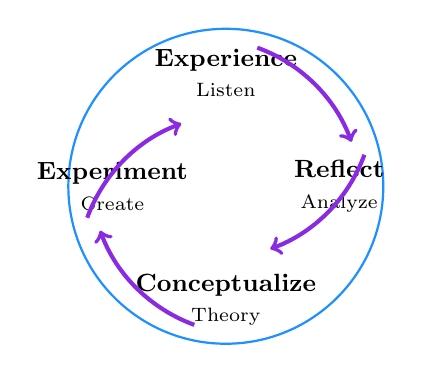
\begin{tikzpicture}[scale=0.8]
    % Circle with 4 quadrants representing Kolb's cycle
    \draw[thick, blue] (0,0) circle (2.5cm);
    
    % Quadrant labels
    \node[align=center, font=\small] at (0,1.8) {\textbf{Experience}\\\scriptsize Listen};
    \node[align=center, font=\small] at (1.8,0) {\textbf{Reflect}\\\scriptsize Analyze};
    \node[align=center, font=\small] at (0,-1.8) {\textbf{Conceptualize}\\\scriptsize Theory};
    \node[align=center, font=\small] at (-1.8,0) {\textbf{Experiment}\\\scriptsize Create};
    
    % Arrows showing cycle direction
    \draw[->, thick, purple, line width=1.5pt] (0.5,2.2) arc (70:20:2.5cm);
    \draw[->, thick, purple, line width=1.5pt] (2.2,0.5) arc (340:290:2.5cm);
    \draw[->, thick, purple, line width=1.5pt] (-0.5,-2.2) arc (250:200:2.5cm);
    \draw[->, thick, purple, line width=1.5pt] (-2.2,-0.5) arc (160:110:2.5cm);
\end{tikzpicture}
\end{center}

\textbf{In Our Program:} Every lesson follows this exact cycle—listen to the song (experience), analyze what you heard (reflect), learn the theory behind it (conceptualize), and recreate it on your machine (experiment).

\subsection*{Constructivism}

\textbf{Who:} Based on work by Jean Piaget (1896-1980), Swiss psychologist who developed cognitive development theory, and Lev Vygotsky (1896-1934), Russian psychologist known for sociocultural theory. Jerome Bruner (1915-2016) further developed constructivist pedagogy in his influential work \textit{The Process of Education} (1960).

\textbf{The Theory:} Learners don't receive knowledge passively—they \greentext{build} it by connecting new information to existing knowledge. Learning is an active process of constructing meaning from experience.

\textbf{The Evidence:} Constructivist approaches show improved problem-solving skills, deeper understanding, and better knowledge transfer compared to traditional instruction. Piaget's and Vygotsky's theories remain foundational in modern educational psychology.

\textbf{In Our Program:} Students build a \bluepurple{repertoire} of patterns—chord progressions, rhythms, techniques—that they continuously remix and reuse. Each new song connects to previous songs, creating a web of musical knowledge.

\subsection*{Enactivism}

\textbf{Who:} Developed by Francisco Varela (1946-2001), Chilean biologist and philosopher, and Humberto Maturana (born 1928) in their seminal work \textit{The Tree of Knowledge} (1987). Extended by philosopher and cognitive scientist Evan Thompson. The theory bridges neuroscience, phenomenology, and Buddhist philosophy.

\textbf{The Theory:} Cognition doesn't happen just in the brain—it arises through physical interaction with the environment. We think through our bodies. Knowledge is enacted through sensorimotor engagement with the world.

\textbf{The Evidence:} Research in embodied cognition shows that physical engagement (especially in music) leads to deeper, more durable learning. Movement and action embed knowledge. Neuroscience confirms that motor, sensory, and cognitive systems are deeply integrated.

\textbf{In Our Program:} Students learn by physically \redtext{playing} The Beat Machine. The tactile experience of pressing drum pads, playing keys, and hitting the loop button makes learning visceral and memorable.

\subsection*{Music as Language}

Just as children learn to speak before they learn to read, musicians should learn to \purple{play} before they learn to notate. Think about language acquisition:

\begin{itemize}[leftmargin=*]
\item Children hear thousands of conversations before speaking their first word
\item They speak fluently for years before learning to read or write
\item Grammar and syntax are learned through \textit{use}, not rules
\item By the time they study "language arts," they already have a massive \bluepurple{vocabulary}
\end{itemize}

Our program applies this same principle to music. Students build their musical vocabulary through \greentext{doing}—playing, creating, listening. Small music theory lessons are introduced in each class, but they don't require any prior understanding and we don't wait to introduce them. Theory becomes the vocabulary for describing what students are actively experiencing in real time.

\begin{center}
\includegraphics[width=0.28\textwidth]{Illustrations/Jamming.png}
\end{center}

\newpage

% PAGE 3: FROM THEORY TO PRACTICE
\section*{From Theory to Practice}

\begin{center}
\includegraphics[width=0.3\textwidth]{Illustrations/Producer.png}
\end{center}

\vspace{0.5cm}

Here's how we translate educational research into an actual learning experience:

\subsection*{The Beat Machine: Your Learning Partner}

\textbf{What It Is:}
\begin{itemize}[leftmargin=*]
\item Full keyboard for melodies, chords, and bass
\item Drum pads for rhythm and percussion
\item Large loop button for seamless recording and playback
\item Built-in speakers for immediate feedback
\item Preloaded with professional sounds and samples
\end{itemize}

\textbf{Why It Matters:}
\begin{itemize}[leftmargin=*]
\item \textbf{Immediate feedback:} Enactivism in action—hear what you play instantly
\item \textbf{Removes technical barriers:} No computer setup, no software installation, no troubleshooting
\item \textbf{Focus stays on music:} Technology serves the learning, not the other way around
\item \textbf{Production-ready:} The skills learned translate directly to any DAW (Ableton, FL Studio, Logic, etc.)
\end{itemize}

\subsection*{The Song-Based Approach}

\textbf{Why Songs You Know:}

Learning happens best when it connects to something familiar. By recreating recognizable songs across all genres and eras—students learn from:

\begin{multicols}{2}
\begin{itemize}[leftmargin=*, itemsep=0pt]
\item The Beatles
\item Stevie Wonder
\item Michael Jackson
\item Drake
\item Beyoncé
\item Daft Punk
\item Billie Eilish
\item The Weeknd
\item Kendrick Lamar
\item Bob Marley
\item Earth, Wind \& Fire
\item Selena
\item Dr. Dre
\item Luis Fonsi
\item Avicii
\item \textit{...and many more!}
\end{itemize}
\end{multicols}

\vspace{0.3cm}

This approach means students:
\begin{itemize}[leftmargin=*]
\item Tap into existing knowledge (constructivism at work)
\item Stay motivated through familiarity and cultural relevance
\item Have a clear goal: "Sound like the \purple{original}"
\item Build confidence by achieving something tangible
\end{itemize}

\textbf{Layer-by-Layer Learning:}

Complex songs can be overwhelming. We break them down:
\begin{enumerate}[leftmargin=*]
\item \textbf{Drums:} Start with rhythm—the foundation of every beat
\item \textbf{Bass:} Add the low end—melody meets rhythm
\item \textbf{Chords:} Build harmony—the emotional core
\item \textbf{Melodies \& Percussion:} Layer in the details
\end{enumerate}

This is \bluepurple{scaffolding} in practice—each layer is an achievable goal that builds confidence and prepares students for the next challenge.

\subsection*{Building Your Musical Vocabulary}

\begin{center}
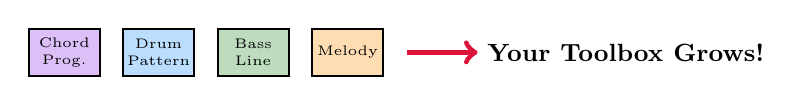
\begin{tikzpicture}[scale=0.6]
    % Toolbox/building blocks illustration
    % Box 1
    \draw[thick, fill=purple!30] (0,0) rectangle (1.5,1);
    \node[align=center, font=\tiny] at (0.75,0.5) {Chord\\Prog.};
    
    % Box 2
    \draw[thick, fill=blue!30] (2,0) rectangle (3.5,1);
    \node[align=center, font=\tiny] at (2.75,0.5) {Drum\\Pattern};
    
    % Box 3
    \draw[thick, fill=green!30] (4,0) rectangle (5.5,1);
    \node[align=center, font=\tiny] at (4.75,0.5) {Bass\\Line};
    
    % Box 4
    \draw[thick, fill=orange!30] (6,0) rectangle (7.5,1);
    \node[align=center, font=\tiny] at (6.75,0.5) {Melody};
    
    % Arrow showing growth
    \draw[->, thick, red, line width=2pt] (8,0.5) -- (9.5,0.5);
    \node[right, font=\small] at (9.5,0.5) {\textbf{Your Toolbox Grows!}};
\end{tikzpicture}
\end{center}

\vspace{0.3cm}

\textbf{The Repertoire Concept:}

Every song teaches patterns: a chord progression, a rhythmic motif, a bassline technique, a drum fill. Over time, students accumulate a \greentext{toolbox} of musical building blocks.

\begin{itemize}[leftmargin=*]
\item After 5 lessons: 10 sections learned (5 songs × 2 sections each)
\item After 10 lessons: 20 sections
\item After 20 lessons: 40 sections in your repertoire
\end{itemize}

These aren't just songs you can play—they're \textbf{patterns you can remix}. That chord progression from "Let It Be"? Use it in your own song. That drum pattern from a hip-hop track? Drop it into a new context.

\textbf{Every Class, Same Structure:}

One of the keys to scalability and consistency is that \redtext{every class follows the exact same structure}. Whether it's your first lesson or your fiftieth, you know what to expect. This consistency allows students to focus on the \textit{content} (the music) rather than the \textit{process} (how the class works). 

Students can join at any time, progress at their own pace, and continuously build their repertoire without worrying about "falling behind." There's no linear curriculum—just an ever-expanding library of skills.

\subsection*{Piano Roll Notation: Setting You Up for Success}

Traditional western notation (treble clef, bass clef, key signatures) is valuable, but it's not designed for modern production. We use \orangetext{piano roll notation}:

\begin{center}
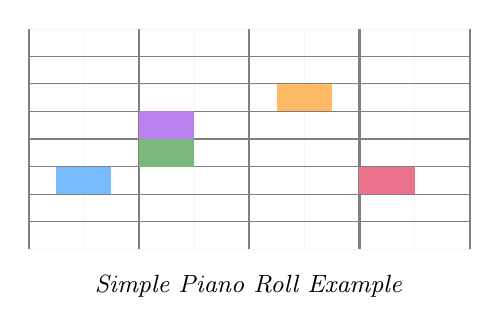
\begin{tikzpicture}[scale=0.7]
    % Piano roll grid illustration
    \draw[lightgray, very thin] (0,0) grid (8,4);
    
    % Horizontal lines for notes
    \foreach \y in {0.5,1,1.5,2,2.5,3,3.5} {
        \draw[gray] (0,\y) -- (8,\y);
    }
    
    % Vertical lines for beats
    \foreach \x in {0,2,4,6,8} {
        \draw[gray, thick] (\x,0) -- (\x,4);
    }
    
    % Example notes as colored rectangles
    \fill[blue!60] (0.5,1) rectangle (1.5,1.5);
    \fill[purple!60] (2,2) rectangle (3,2.5);
    \fill[green!60] (2,1.5) rectangle (3,2);
    \fill[orange!60] (4.5,2.5) rectangle (5.5,3);
    \fill[red!60] (6,1) rectangle (7,1.5);
    
    \node[below] at (4,-0.3) {\small\textit{Simple Piano Roll Example}};
\end{tikzpicture}
\end{center}

\begin{itemize}[leftmargin=*]
\item \textbf{Visual \& intuitive:} High notes are literally higher on the page
\item \textbf{Rhythm is clear:} Grid-based timing makes syncopation obvious
\item \textbf{Direct transfer:} Every DAW uses piano roll—students leave class production-ready
\item \textbf{Lower barrier:} No need to memorize clefs or key signatures before making music
\end{itemize}

We're not replacing traditional music education—we're \purple{expanding} it for the modern creator.

\newpage

% PAGE 4: ANATOMY OF A CLASS
\section*{Anatomy of a Class}

\begin{center}
\includegraphics[width=0.3\textwidth]{Illustrations/BeatMaker.png}
\end{center}

\vspace{0.3cm}

Here's what happens in every 60-75 minute lesson:

\begin{center}
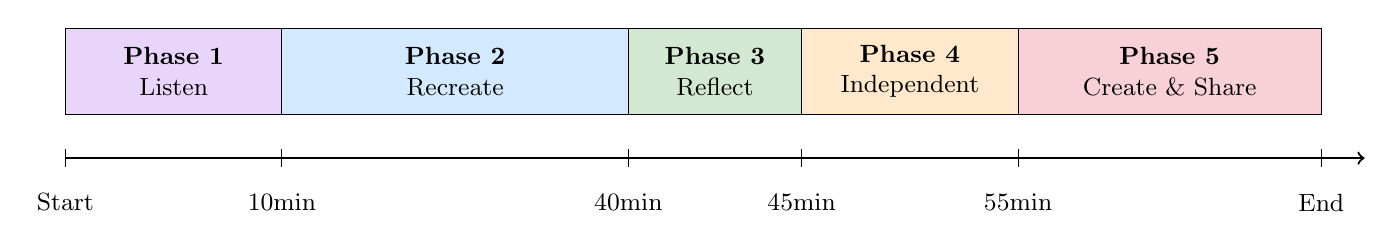
\begin{tikzpicture}[scale=1.1]
    % Timeline
    \draw[thick, ->] (0,0) -- (15,0);
    
    % Phase markers
    \foreach \x/\label in {0/Start, 2.5/10min, 6.5/40min, 8.5/45min, 11/55min, 14.5/End} {
        \draw (\x,0.1) -- (\x,-0.1);
        \node[below] at (\x,-0.3) {\small\label};
    }
    
    % Phase boxes - wider
    \draw[fill=purple!20] (0,0.5) rectangle (2.5,1.5);
    \node[align=center, font=\small] at (1.25,1) {\textbf{Phase 1}\\Listen};
    
    \draw[fill=blue!20] (2.5,0.5) rectangle (6.5,1.5);
    \node[align=center, font=\small] at (4.5,1) {\textbf{Phase 2}\\Recreate};
    
    \draw[fill=green!20] (6.5,0.5) rectangle (8.5,1.5);
    \node[align=center, font=\small] at (7.5,1) {\textbf{Phase 3}\\Reflect};
    
    \draw[fill=orange!20] (8.5,0.5) rectangle (11,1.5);
    \node[align=center, font=\small] at (9.75,1) {\textbf{Phase 4}\\Independent};
    
    \draw[fill=red!20] (11,0.5) rectangle (14.5,1.5);
    \node[align=center, font=\small] at (12.75,1) {\textbf{Phase 5}\\Create \& Share};
\end{tikzpicture}
\end{center}

\vspace{0.5cm}

\subsection*{Phase 1: Listen \& Analyze \texorpdfstring{\textcolor{purple}{(10 minutes)}}{(10 minutes)}}
\textit{Kolb Stage: Concrete Experience}

\begin{itemize}[leftmargin=*]
\item \textbf{Active listening:} Play the song—focus on different elements with each listen
\item \textbf{Historical context:} Learn about the artist, era, and cultural significance
\item \textbf{Student analysis:} Open discussion—What do you hear? How does it make you feel? What instruments stand out?
\item \textbf{Comparables:} Connect this song to others you know—patterns emerge
\end{itemize}

\subsection*{Phase 2: Deconstruct \& Recreate \texorpdfstring{\textcolor{blue}{(30 minutes)}}{(30 minutes)}}
\textit{Kolb Stages: Reflective Observation + Abstract Conceptualization}

\textbf{Layer-by-Layer Breakdown:}
\begin{enumerate}[leftmargin=*]
\item Teacher demonstrates the first layer (usually drums) on The Beat Machine
\item Students practice on their own machines, working to match the original
\item Teacher circulates, providing feedback and "signing off" when each student has it right
\item Repeat for each layer: bass, chords, percussion, melody
\end{enumerate}

\textbf{Extension Activities for Fast Finishers:}
\begin{itemize}[leftmargin=*]
\item \greentext{Sketch the layer} on a blank piano roll template—building notation skills
\item Free creative time to experiment with variations of what they've learned
\end{itemize}

\textbf{Theory Integration:}

As each layer is learned, the teacher introduces small music theory lessons:
\begin{itemize}[leftmargin=*]
\item "This is a I-V-vi-IV chord progression—you'll hear it everywhere"
\item "Notice how the kick drum hits on beats 1 and 3? That's the backbone"
\item "The bass is playing the root notes of the chords—that's what makes it sound 'locked in'"
\end{itemize}

Theory feels \bluepurple{relevant} because it's tied directly to what students are actively playing. It's not abstract—it's the language describing their experience in real time.

\subsection*{Phase 3: Metacognition Break \texorpdfstring{\textcolor{green}{(5 minutes)}}{(5 minutes)}}
\textit{Kolb Stage: Reflective Observation}

Before recreating the beat independently, we pause:

\begin{itemize}[leftmargin=*]
\item "What did you \purple{learn} today?"
\item "Which techniques could you use in your own music?"
\item "What was challenging? What clicked?"
\item "How does this song compare to others we've learned?"
\end{itemize}

This reflection primes students for success in the next phase and builds \redtext{metacognitive awareness}—understanding their own learning process.

\subsection*{Phase 4: Independent Recreation \texorpdfstring{\textcolor{orange}{(10 minutes)}}{(10 minutes)}}
\textit{Kolb Stage: Active Experimentation}

\textbf{The Challenge:} Recreate the full beat—all layers, start to finish—using only your memory, notes, and piano roll sketches.

\begin{itemize}[leftmargin=*]
\item No teacher help during this phase
\item Pure application of what you've learned
\item Builds confidence and independence
\end{itemize}

This is where students realize: \textit{"I can actually do this."}

\subsection*{Phase 5: Original Creation \& Share \texorpdfstring{\textcolor{red}{(15-20 minutes)}}{(15-20 minutes)}}
\textit{Kolb Stage: Active Experimentation}

\textbf{Free Creation Time:}

Now the real magic happens. Students compose \greentext{original beats} using techniques from today's lesson—and any previous lessons:

\begin{itemize}[leftmargin=*]
\item Use today's chord progression with a different rhythm
\item Combine today's drums with last week's bassline
\item Experiment, take risks, make something \textit{yours}
\end{itemize}

\textbf{Share \& Celebrate:}

Students play their creations for the class. This is where community forms:
\begin{itemize}[leftmargin=*]
\item Peer feedback and recognition
\item Hearing different interpretations of the same techniques
\item Building confidence as a \orangetext{creator}, not just a learner
\end{itemize}

\vspace{0.5cm}

\subsection*{Class Formats}

\begin{center}
\includegraphics[width=0.3\textwidth]{Illustrations/Band.png}
\end{center}

\begin{itemize}[leftmargin=*]
\item \textbf{In-Person:} Full hands-on experience with The Beat Machine, collaborative energy, direct teacher support
\item \textbf{Online:} Same structure, same learning—students use their own Beat Machines at home via video platform
\end{itemize}

\newpage

% PAGE 5: WHAT STUDENTS GAIN
\section*{What Students Gain}

\begin{center}
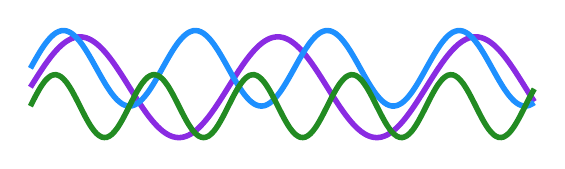
\begin{tikzpicture}[scale=0.8]
    % Sound wave illustration
    \draw[purple, line width=2pt, domain=0:8, samples=100, smooth] 
        plot (\x, {0.8*sin(2*\x r)});
    \draw[blue, line width=2pt, domain=0:8, samples=100, smooth] 
        plot (\x, {0.6*sin(3*\x r) + 0.3});
    \draw[green, line width=2pt, domain=0:8, samples=100, smooth] 
        plot (\x, {0.5*sin(4*\x r) - 0.3});
\end{tikzpicture}
\end{center}

\vspace{0.3cm}

This program develops far more than just beatmaking skills. Here's what students walk away with:

\subsection*{Musical Skills 

\begin{tikzpicture}[baseline=-0.5ex, scale=0.15]
    \fill[purple] (0,0) circle (0.8);
    \draw[white, line width=1pt] (-0.3,-0.3) -- (-0.3,0.3) -- (0.3,0.3) -- (0.3,-0.3);
\end{tikzpicture}}

\begin{itemize}[leftmargin=*]
\item \textbf{Practical production ability:} Students leave ready to use any DAW—Ableton, FL Studio, Logic, GarageBand. No additional "translation" needed.
\item \textbf{Ear training:} Recognize chord progressions, rhythmic patterns, and production techniques in \textit{any} song. Music becomes a language you understand.
\item \textbf{Music theory:} Understanding rooted in \purple{application}, not abstraction. Theory is the vocabulary for describing what you already know how to play.
\item \textbf{Growing repertoire:} A library of patterns and techniques that expands with every lesson. By lesson 20, students have 40+ sections they can play and remix.
\end{itemize}

\subsection*{Cognitive \& Creative Skills 

\begin{tikzpicture}[baseline=-0.5ex, scale=0.15]
    \fill[blue] (0,0) circle (0.8);
    \draw[white, line width=1.5pt] (-0.4,0.4) -- (-0.1,0) -- (0.4,0.5);
\end{tikzpicture}}

\begin{itemize}[leftmargin=*]
\item \textbf{Problem-solving:} Breaking complex challenges (songs) into manageable parts (layers) is a transferable skill that applies far beyond music.
\item \textbf{Pattern recognition:} Seeing connections across different songs, genres, and styles. Recognizing that "this chord progression is the same as that one" builds analytical thinking.
\item \textbf{Creative confidence:} Students move from \textit{"I can't make music"} to \bluepurple{"Listen to what I made!"} That shift in identity is powerful.
\item \textbf{Metacognitive awareness:} Understanding \textit{how} you learn makes you a better learner in every domain, not just music.
\end{itemize}

\subsection*{Social-Emotional Skills 

\begin{tikzpicture}[baseline=-0.5ex, scale=0.15]
    \fill[red] (0,0) circle (0.8);
    \draw[white, line width=1.5pt] (-0.3,0.2) .. controls (-0.3,-0.1) and (0.3,-0.1) .. (0.3,0.2);
    \fill[white] (-0.25,0.3) circle (0.15);
    \fill[white] (0.25,0.3) circle (0.15);
\end{tikzpicture}}

\begin{itemize}[leftmargin=*]
\item \textbf{Collaboration:} Peer teaching, learning together, and sharing creations build community and communication skills.
\item \textbf{Perseverance:} Working through challenges to nail each layer teaches grit and resilience.
\item \textbf{Self-expression:} Music becomes an outlet for creativity, emotion, and personal voice.
\item \textbf{Cultural literacy:} Learning the history behind songs builds understanding of different eras, cultures, and movements.
\end{itemize}

\vspace{1.5cm}

\subsection*{Why This Matters}

Music education shouldn't be a luxury for those who can afford private lessons or have access to expensive equipment. It shouldn't require years of practice before you can make something that sounds good. And it shouldn't feel disconnected from the music students actually listen to and love.

\begin{center}
\includegraphics[width=0.35\textwidth]{Illustrations/DJ.png}
\end{center}

\textbf{Beatmaking: Learn By Doing} makes music creation \greentext{accessible}, \redtext{immediate}, and \bluepurple{empowering}. Students leave every class having \textit{made something}—and that sense of accomplishment builds momentum.

Whether students go on to become professional producers or simply gain a deeper appreciation for music, they've developed skills, confidence, and creativity that will serve them for life.

\newpage

% PAGE 6: FAQ
\section*{Ready to Start Your Musical Journey?}

\begin{center}

\begin{tikzpicture}[scale=0.5]
    % Stars decoration - right side up
    \foreach \x/\col in {0/purple, 2/blue, 4/orange, 6/green, 8/red} {
        \fill[\col] (\x,1.4) -- (\x-0.2,0.8) -- (\x-0.6,0.8) -- (\x-0.3,0.4) -- (\x-0.4,0) -- (\x,0.4) -- (\x+0.4,0) -- (\x+0.3,0.4) -- (\x+0.6,0.8) -- (\x+0.2,0.8) -- cycle;
    }
\end{tikzpicture}
\end{center}

\vspace{0.5cm}

\subsection*{Who Is This For?}

This program is designed for \textbf{everyone}, regardless of where you are in your musical journey:

\begin{itemize}[leftmargin=*]
\item \textbf{Complete beginners:} No musical experience required—start from scratch and make music from day one
\item \textbf{Instrument players:} You play guitar, piano, or another instrument but want to learn \purple{production}? Perfect. Translate your musical knowledge into beats.
\item \textbf{Experienced producers:} Been producing for years? Build your \bluepurple{repertoire} with new patterns, progressions, and techniques from diverse genres
\item \textbf{Aspiring learners:} Always wanted to learn piano or guitar but found traditional lessons intimidating? This is your path—learn music through \greentext{creation}, not repetition
\item \textbf{DJs \& performers:} Want to make your own tracks instead of just playing others'? Learn production fundamentals that translate directly to the stage
\item \textbf{Professional track:} This is the perfect foundation for becoming a \redtext{professional producer} or \redtext{DJ}—you'll leave with real skills, a portfolio of techniques, and the confidence to create commercially
\end{itemize}

\textbf{Practical Details:}
\begin{itemize}[leftmargin=*]
\item \textbf{Age range:} 8 to 80—this program works for all ages
\item \textbf{Equipment:} The Beat Machine provided for in-person classes; purchase/rental options available for online learning
\item \textbf{Commitment:} Classes meet weekly; students build repertoire continuously over time
\end{itemize}

\subsection*{Frequently Asked Questions}

\textbf{Q: Do I need to know how to read music?}

A: Not at all! We use piano roll notation, which is visual, intuitive, and sets you up for modern music production. No treble clef required.

\vspace{0.4cm}

\textbf{Q: What if I've never made music before?}

A: Perfect! This program is designed for beginners. We start from the ground up, and by the end of your first class, you'll have made a beat.

\vspace{0.4cm}

\textbf{Q: What styles of music will we learn?}

A: We cover a wide range—hip-hop, R\&B, pop, rock, electronic, soul, and more. One week we might recreate "Come Together" by The Beatles; the next week, a modern hip-hop track. The patterns and techniques transfer across genres.

\vspace{0.4cm}

\textbf{Q: Will I be able to make my own songs?}

A: Absolutely. Every lesson includes time for \purple{original creation}. You'll build the skills and confidence to compose independently—and those skills grow with every class you take.

\vspace{0.4cm}

\textbf{Q: What happens after I complete the program?}

A: There's no "completion"—students can continue taking classes indefinitely, building an ever-expanding repertoire. The structure is designed to be \bluepurple{scalable}. You can take 10 classes or 100 classes; each one adds to your musical vocabulary.

\vspace{0.4cm}

\textbf{Q: Can I use what I learn on other equipment/software?}

A: Yes! The skills translate directly to any DAW (Ableton, FL Studio, Logic, GarageBand, etc.). Piano roll is piano roll, and the patterns you learn are universal.

\vspace{0.4cm}

\textbf{Q: How is this different from traditional music lessons?}

A: Traditional lessons often focus on notation, technique, and classical repertoire before students get to \textit{create}. We flip that: students create from day one, building practical skills that lead to immediate results. Theory is introduced alongside practice in every class.

\vspace{1cm}

\begin{center}
\includegraphics[width=0.4\textwidth]{Illustrations/DJShow.png}
\end{center}

\vspace{0.5cm}

\begin{center}
\rule{0.8\textwidth}{0.5pt}

\vspace{0.5cm}

\Large\textbf{Beatmaking: Learn By Doing}

\vspace{0.3cm}

\normalsize Music education for the modern \orangetext{creator}

\vspace{0.5cm}

\small Designed by \textbf{Connor Puhala}

\small Berklee College of Music Graduate \& Professional Music Educator

\vspace{0.8cm}

\normalsize
\href{https://www.makebeatsanywhere.com/}{www.makebeatsanywhere.com} \\[0.2cm]
\href{mailto:connor@makebeatsanywhere.com}{connor@makebeatsanywhere.com} \\[0.2cm]
\href{https://www.instagram.com/the_beat_machine_}{@the\_beat\_machine\_}

\vspace{0.5cm}

\rule{0.8\textwidth}{0.5pt}
\end{center}

\end{document}
